\documentclass[a4j, titlepage]{jsarticle}
\usepackage[dvipdfmx]{graphicx}
\usepackage{amsmath,ascmac,amsthm, amssymb}
\usepackage{amsfonts,latexsym,mathtools}
\usepackage{bm}
\usepackage{algorithm,algorithmic}
\usepackage{listings}
\usepackage{empheq}
\lstset{
    language={C},
    basicstyle={\small\ttfamily},
    identifierstyle={\small},
    commentstyle={\small\itshape},
    keywordstyle={\small\bfseries},
    ndkeywordstyle={\small},
    stringstyle={\small\ttfamily},
    frame={tb},
    breaklines=true,
    columns=[l]{fullflexible},
    numbers=left,
    xrightmargin=0zw,
    xleftmargin=3zw,
    numberstyle={\scriptsize},
    stepnumber=1,
    numbersep=1zw,
    lineskip=-0.5ex
}
\renewcommand{\lstlistingname}{リスト}
\renewcommand{\lstlistlistingname}{リスト目次}

\numberwithin{equation}{section}
%\setcounter{tocdepth}{3}

\begin{document}
\begin{titlepage}
    \begin{center}
        {\Large 令和四年度後期 数理工学実験 課題レポート}

        \vspace*{180truept}

        {\Huge 関数の補間と数値積分}

        \vspace{160truept}

        {\Large 情報学科2回生 平田蓮}

        \vspace{10truept}

        {\large 学生番号: 1029342830}

        \vspace{60truept}

        {\large 実験日: 11月8, 14, 15, 28日}

        \vspace{10truept}

        {\large 実験場所: 京都大学工学部総合校舎数理計算機室}

        \vspace{60truept}

        {\large 12月5日 提出}
    \end{center}
\end{titlepage}

\tableofcontents
\clearpage

\section{目的}
    本実験では数値積分を扱う。
    数値積分は理学・工学のさまざまな場面で現れるが、
    これを解析的に解くことは特別な場合を除いて非常に困難であるため、
    本実験では関数補間を用いて近似的に積分の数値解を得ることを目標とする。

\section{原理}
    式(\ref{equ:int})に示す積分を解くことを考える。
    本節では、のちに行う課題で用いる積分法について記す。

    \begin{equation}
        \int_a^bf(x)\mathrm{d}x \label{equ:int}
    \end{equation}

    \subsection{Newton-Cotes積分公式}
        Newton-Cotes積分公式は最も基本的な積分公式である。
        これは、Lagrange補間を用いるため、
        それについても以下に記す。

        \subsubsection{Lagrange補間}
            $f(x)$を$n-1$次多項式$P(x)$で表すことを考える。
            $x\in[a,b]$から$n$点$x_1,x_2,\cdots,x_n$を選び、
            $P(x_i)=f(x_i)$となるように$P(x)$を構成する。
            $P(x)$の$i$次の係数を$a_i$とすると、
            各$i=0,1,\cdots,n-1$について、
            \begin{equation*}
                a_0 + a_1x_i + \cdots + a_{n-1}x_i^{n-1} = f(x_i)
            \end{equation*}
            を満たせば良い。これは次のように書き直せる。
            \begin{equation*}
                \begin{pmatrix}
                    1 & x_1 & \cdots & x_1^{n-1} \\
                    1 & x_2 & \cdots & x_2^{n-1} \\
                    \vdots & \vdots & \ddots & \vdots \\
                    1 & x_n & \cdots & x_n^{n-1}
                \end{pmatrix}\begin{pmatrix}
                    a_0 \\
                    a_1 \\
                    \vdots \\
                    a_{n-1}
                \end{pmatrix} = \begin{pmatrix}
                    f(x_1) \\
                    f(x_2) \\
                    \vdots \\
                    f(x_n)
                \end{pmatrix}
            \end{equation*}
            これの係数行列の行列式は、
            \begin{equation*}
                \begin{vmatrix}
                    1 & x_1 & \cdots & x_1^{n-1} \\
                    1 & x_2 & \cdots & x_2^{n-1} \\
                    \vdots & \vdots & \ddots & \vdots \\
                    1 & x_n & \cdots & x_n^{n-1}
                \end{vmatrix} = \prod_{i=1}^n\prod_{j=i+1}^n(x_i-x_j)\neq 0
            \end{equation*}
            となるため、条件を満たす$P(x)$は一意に定まることがわかり、それは
            \begin{equation}
                P(x) = \sum_{i=1}^n\frac{\displaystyle\prod_{j=1,j\neq i}^n (x-x_j)}{\displaystyle\prod_{j=1,j\neq i}^n (x_i-x_j)}f(x_i) \label{equ:lagrange}
            \end{equation}
            と書ける。

        \subsubsection{Newton-Cotes積分公式}
            分点$\{x_i\}$を用いてLagrange補間を行い、
            式(\ref{equ:int})の積分値を計算する。
            式(\ref{equ:int})を書き直すと、
            \begin{eqnarray*}
                \int_a^bf(x)\mathrm{d}x &=& \int_a^bP(x)\mathrm{d}x \\
                &=& \int_a^b\sum_{i=1}^n\frac{\displaystyle\prod_{j=1,j\neq i}^n (x-x_j)}{\displaystyle\prod_{j=1,j\neq i}^n (x_i-x_j)}f(x_i)\mathrm{d}x \\
                &=& \sum_{i=1}^nf(x_i)\int_a^b\frac{\displaystyle\prod_{j=1,j\neq i}^n (x-x_j)}{\displaystyle\prod_{j=1,j\neq i}^n (x_i-x_j)}\mathrm{d}x
            \end{eqnarray*}
            を得る。これをNewton-Cotes積分公式と呼ぶ。
            この公式は、分点の取り方によって変化するが、
            本実験では以下に示す3種類を使う。

            \paragraph{中点公式}
                一つの分点$x_1 = \displaystyle\frac{a + b}{2}$のみを考える。

                $\displaystyle\int_a^b\frac{\displaystyle\prod_{j=1,j\neq i}^n (x-x_j)}{\displaystyle\prod_{j=1,j\neq i}^n (x_i-x_j)}\mathrm{d}x=\int_a^b\mathrm{d}x=b-a$となるので、
                $\displaystyle\int_a^bf(x)\mathrm{d}x\approx(b-a)f(x_1)$と近似できる。
                これを中点公式という。

            \paragraph{台形公式}
                二つの分点$x_1 = a, x_2 = b$を考える。

                $\displaystyle\int_a^b\frac{\displaystyle\prod_{j=1,j\neq i}^n (x-x_j)}{\displaystyle\prod_{j=1,j\neq i}^n (x_i-x_j)}\mathrm{d}x=\int_a^b\frac{1}{2}\mathrm{d}x=\frac{b-a}{2}$となるので、
                $\displaystyle\int_a^bf(x)\mathrm{d}x\approx\frac{b-a}{2}\{f(x_1)+f(x_2)\}$と近似できる。
                これを台形公式という。

            \paragraph{Simpson公式}
                三つの分点$x_1 = a, x_2 = \displaystyle\frac{b-a}{2}, x_3 = b$を考える。

                \begin{equation*}
                    \int_a^b\frac{\displaystyle\prod_{j=1,j\neq i}^n (x-x_j)}{\displaystyle\prod_{j=1,j\neq i}^n (x_i-x_j)}\mathrm{d}x=\begin{cases}
                        \displaystyle\frac{b-a}{6} & i=1,3 \\
                        \displaystyle\frac{2}{3}(b-a) & i=2
                    \end{cases}
                \end{equation*}
                となるので、
                $\displaystyle\int_a^bf(x)\mathrm{d}x\approx\frac{b-a}{6}\{f(x_1)+4f(x_2)+f(x_3)\}$と近似できる。
                これを台形公式という。

        \subsubsection{複合公式}
            前節で述べた公式は、$x\in[a,b]$において$f(x)$を定数、一次関数、二次関数で近似して得ているため、
            その実際の値との誤差は$|b-a|$に比例して大きくなってしまう。
            そこで、実際の積分範囲を十分に細かく分割し、
            それぞれに積分公式を用いて計算を行うのが一般的である。
            
            $x_i=a+ih \ \left(i=0,1,\cdots,n, \ \displaystyle h=\frac{b-a}{n}\right)$として、
            $[a_i,a_{i+1}]$にそれぞれの積分公式を適用すると、次のように書ける。

            \paragraph{中点複合公式}
                \begin{equation}
                    \int_a^bf(x)\mathrm{d}x\approx h\sum_{i=0}^{n-1}f\left(\frac{x_i+x_{i+1}}{2}\right) \label{equ:midpoint}
                \end{equation}

            \paragraph{台形複合公式}
                \begin{equation}
                    \int_a^bf(x)\mathrm{d}x\approx\frac{h}{2}\left\{f(x_0) + \sum_{i=1}^{n-1}f(x_i) + f(x_n)\right\} \label{equ:trapezoid}
                \end{equation}

            \paragraph{Simpson複合公式}
                \begin{equation}
                    \int_a^bf(x)\mathrm{d}x\approx\frac{h}{6}\left\{f(x_0) + \sum_{i=1}^{n-1}f(x_i) + f(x_n) + 4\sum_{i=0}^{n-1}f\left(\frac{x_i+x_{i+1}}{2}\right)\right\} \label{equ:simpson}
                \end{equation}

    \subsection{Gauss型積分公式}
        二つの関数$f(x),g(x)$の内積$(f,g)$を以下で定義する。
        \begin{equation*}
            (f,g)=\int_{-1}^1f(x)g(x)\mathrm{d}x
        \end{equation*}
        これが0となるとき、二つの関数は直交するという。
        任意の$n-1$次多項式と直交する$n$次式多項式$P_n(x)$が存在することが知られ、
        これをLegendre多項式と呼ぶ。

        $f(x)$を$P_n(x)$で割った商を$Q(x)$,余りを$R(x)$とすると、
        \begin{equation*}
            f(x) = P_n(x)Q(x)+R(x)
        \end{equation*}
        と書ける。ここで、$Q(x),R(x)$は$n-1$次多項式であることに注意する。
        $a=-1,b=1$として式(\ref{equ:int})を解くことを考えると、
        \begin{eqnarray*}
            \int_{-1}^1f(x)\mathrm{d}x &=& \int_{-1}^1\{P_n(x)Q(x)+R(x)\}\mathrm{d}x \\
            &=& \int_{-1}^1R(x)\mathrm{d}x \ (\because P_n(x)とQ(x)は直交)
        \end{eqnarray*}
        と書ける。
        ここで、$R(x)$のLagrange補間は$R(x)$に等しいため、
        \begin{equation*}
            \int_{-1}^1R(x)\mathrm{d}x = \sum_{i=1}^nR(x_i)\int_{-1}^1\frac{\displaystyle\prod_{j=1,j\neq i}^n (x-x_j)}{\displaystyle\prod_{j=1,j\neq i}^n (x_i-x_j)}\mathrm{d}x
        \end{equation*}
        となり、$\{x_i\}$に$P_n(x)$の零点を用いると、上の結果と合わせて、
        \begin{equation*}
            \int_{-1}^1f(x)\mathrm{d}x = \sum_{i=1}^nf(x_i)\int_{-1}^1\frac{\displaystyle\prod_{j=1,j\neq i}^n (x-x_j)}{\displaystyle\prod_{j=1,j\neq i}^n (x_i-x_j)}\mathrm{d}x
        \end{equation*}
        を得る。これをGauss型積分公式と呼ぶ。
        これは積分範囲が$[-1,1]$であるが、
        適切に変数変換を行うことで任意の範囲で積分を行うことが可能である。

        \subsubsection{複合公式}
            Gauss型積分公式も、一般的に複合公式を作成して計算を行う。
            $x_i=a+ih \ \left(i=0,1,\cdots,n, \ \displaystyle h=\frac{b-a}{n}\right)$
            とすると、
            \begin{equation*}
                \int_a^bf(x)\mathrm{d}x=\sum_{i=0}^{n-1}\int_{x_i}^{x_{i+1}}f(x)\mathrm{d}x
            \end{equation*}
            である。$\displaystyle y = 2\frac{x-x_i}{x_{i+1}-x_i}-1$と変数変換を行うと、
            $x\in[x_i,x_{i+1}]$は$y\in[-1,1]$となり、Gauss型積分公式を適用できる。
            $M$次Legendre多項式を用いたGauss型積分公式を適用すると、
            \begin{eqnarray}
                \int_a^bf(x)\mathrm{d}x &=& \sum_{i=0}^{n-1}\int_{x_i}^{x_{i+1}}f(x)\mathrm{d}x \nonumber \\
                &=& \sum_{i=0}^{n-1}\int_{-1}^{1}f\left(\frac{(y+1)(x_{i+1}-x_i)}{2}+x_i\right)\frac{x_{i+1}-x_i}{2}\mathrm{d}y \nonumber \\
                &\approx& \sum_{i=0}^{n-1}\sum_{m=1}^{M}w_mf\left(\frac{(y_m+1)(x_{i+1}-x_i)}{2}+x_i\right)\frac{x_{i+1}-x_i}{2} \label{equ:gauss}
            \end{eqnarray}
            と書ける。
            ここで、$y_m$はLegendre多項式の$m$番目の零点、
            $w_m$は$M$次Lagrange補間の$m-1$次の係数である。

\section{課題}
    \subsection{課題4.2}
        区間$[a,b]$における$n+1$個の分点を以下で定める:
        \begin{equation*}
            x_i = a + \frac{b-a}{n}i \ (i = 0, 1, \cdots, n)
        \end{equation*}

        \subsubsection{}
            以下に示す三つの関数について、$x_i$における値を求め、
            $n=2,4,8,16$としてLagrange補間で$n$次多項式$P(x)$を求める。

            \begin{itemize}
                \item $f_1(x) = \ln x \ (x \in [1, 2])$
                \item $f_2(x) = \displaystyle\frac{1}{x^3} \ (x \in [0.1, 2])$
                \item $f_3(x) = \displaystyle\frac{1}{1+25x^2} \ (x \in [-1, 1])$
            \end{itemize}

            作成したコードをリスト\ref{src:lagrange}, \ref{src:f1}, \ref{src:f2}, \ref{src:f3}に示す。

            \begin{lstlisting}[caption=式(\ref{equ:lagrange})の実装, label=src:lagrange]
#include <iostream>
#include <vector>

class Lagrange {
private:
    const double (*f)(const double);
    const double start, end;
    const int n;

    std::vector<double> xs;

    void calculate_points() {
        for (int i = 0; i <= this->n; i++) {
            this->xs[i] = this->start + (this->end - this->start) / (double)n * (double)i;
        }
    }

    const double l(
        const int i,
        const double x
    ) {
        double return_value = 1;
        for (int j = 0; j <= this->n; j++) {
            if (j == i) {
                continue;
            }

            return_value *= (x - this->xs[j]) / (this->xs[i] - this->xs[j]);
        }

        return return_value;
    }

    const double P(const double x) {
        double return_value = 0;
        for (int i = 0; i <= this->n; i++) {
            return_value += f(this->xs[i]) * this->l(i, x);
        }

        return return_value;
    }

public:
    Lagrange(
        const double (*f)(const double),
        const double start,
        const double end,
        const int n
    ) : f(f), start(start), end(end), n(n), xs(n + 1, 0) {
        this->calculate_points();
    }

    void print_interpolated(
        const double dx
    ) {
        for (double x = this->start; x <= this->end; x += dx) {
            std::cout << x << " " << this->P(x) << std::endl;
        }
    }
};
            \end{lstlisting}
            \begin{lstlisting}[caption=$f_1(x)$の実装, label=src:f1]
#include <cmath>

inline constexpr double f1(const double x) {
    return log(x);
}
            \end{lstlisting}
            \begin{lstlisting}[caption=$f_2(x)$の実装, label=src:f2]
inline constexpr double f2(const double x) {
    return 1.0 / x / x / x;
}
            \end{lstlisting}
            \begin{lstlisting}[caption=$f_3(x)$の実装, label=src:f3]
inline constexpr double f3(const double x) {
    return 1.0 / (1.0 + 25 * x * x);
}
            \end{lstlisting}

            \paragraph{結果・考察}
                作成したグラフを図\ref{fig:f1}, \ref{fig:f2}, \ref{fig:f3}に示す。
                
                \begin{figure}[h]
                    \centering
                    \includegraphics[width=0.8\hsize]{kadai2/1/f1.pdf}
                    \caption{$f_1(x)$のLagrange補間}
                    \label{fig:f1}
                \end{figure}
                \begin{figure}[h]
                    \centering
                    \includegraphics[width=0.8\hsize]{kadai2/1/f2.pdf}
                    \caption{$f_2(x)$のLagrange補間}
                    \label{fig:f2}
                \end{figure}
                \begin{figure}[h]
                    \centering
                    \includegraphics[width=0.8\hsize]{kadai2/1/f3.pdf}
                    \caption{$f_3(x)$のLagrange補間}
                    \label{fig:f3}
                \end{figure}

                $f_1(x)$の近似は、$n=2$の時点で
                人の目では誤差がわからない程度の非常に高い精度で行われていることがわかり、
                $f_1(x)$は$x\in[1,2]$において二次関数に近い形をとっていることがわかる。
                一方、$f_{2,3}(x)$は$n$が増加するにつれ$x=0$付近から徐々に
                近似の精度が上がっていることがわかる。
                これは、Lagrange補間は$n-1$次までのマクローリン展開を
                行っているためであると考えられる。

        \subsubsection{}
            以下に示す四つの関数について、それぞれの範囲における定積分を考える。
            \begin{itemize}
                \item $f_4(x) = \displaystyle\frac{1}{x} \ (x\in[1,2])$
                \item $f_5(x) = e^{5x} \ (x\in[-1,1])$
                \item $f_6(x) = 1 + \sin x \ (x\in[0,\pi])$
                \item $f_7(x) = 1 + \sin x \ (x\in[0,2\pi])$
            \end{itemize}

            これらの積分を中点複合公式、台形複合公式、Simpson複合公式で計算する。
            分割数$n$における計算結果を$I_n$とし、$n\rightarrow\infty$において
            これが理論値$\displaystyle\int_a^bf_i(x)\mathrm{d}x$に収束するか否かを調べる。

            なお、それぞれの理論値は以下に示す通りである。
            \begin{itemize}
                \item $\displaystyle\int_1^2f_4(x)\mathrm{d}x = \ln 2 \approx 0.693147$
                \item $\displaystyle\int_{-1}^1f_5(x)\mathrm{d}x = \frac{e^5-e^{-5}}{5} \approx 29.6813$
                \item $\displaystyle\int_0^{\pi}f_6(x)\mathrm{d}x = 2 + \pi \approx 5.14159$
                \item $\displaystyle\int_0^{2\pi}f_7(x)\mathrm{d}x = 2\pi \approx 6.28319$
            \end{itemize}

            作成したコードをリスト\ref{src:midpoint}, \ref{src:trapezoid}, \ref{src:simpson}, \ref{src:f4}, \ref{src:f5}, \ref{src:f6}に示す。
            \begin{lstlisting}[caption=式(\ref{equ:midpoint})の実装, label=src:midpoint]
const double midpoint(
    const double (*f)(const double),
    const double start,
    const double end,
    const int n
) {
    const double h = (end - start) / (double)n;
    double lastx = start;
    double return_value = 0;
    for (double x = lastx + h; x <= end; lastx = x, x += h) {
        return_value += f((lastx + x) / 2.0);
    }

    return return_value * h;
}
            \end{lstlisting}
            \begin{lstlisting}[caption=式(\ref{equ:trapezoid})の実装, label=src:trapezoid]
const double trapezoid(
    const double (*f)(const double),
    const double start,
    const double end,
    const int n
) {
    const double h = (end - start) / (double)n;
    double return_value = 0;
    for (double x = start + h; x < end; x += h) {
        return_value += 2.0 * f(x);
    }

    return (f(start) + return_value + f(end)) * h / 2.0;
}
            \end{lstlisting}
            \begin{lstlisting}[caption=式(\ref{equ:simpson})の実装, label=src:simpson]
const double simpson(
    const double (*f)(const double),
    const double start,
    const double end,
    const int n
) {
    const double h = (end - start) / (double)n;
    double return_value = f(start) + f(end);
    double lastx = start;
    for (double x = start + h; x <= end; lastx = x, x += h) {
        return_value += 2.0 * f(lastx) + 4 * f((lastx + x) / 2.0);
    }

    return return_value * h / 6.0;
}
            \end{lstlisting}
            \begin{lstlisting}[caption=$f_4(x)$の実装, label=src:f4]
inline constexpr double f4(const double x) {
    return 1.0 / x;
}
            \end{lstlisting}
            \begin{lstlisting}[caption=$f_5(x)$の実装, label=src:f5]
#include <cmath>

inline constexpr double f5(const double x) {
    return exp(5.0 * x);
}
            \end{lstlisting}
            \begin{lstlisting}[caption=$f_{6,7}(x)$の実装, label=src:f6]
#include <cmath>

inline constexpr double f6(const double x) {
    return 1.0 + sin(x);
}
            \end{lstlisting}

            \paragraph{結果・考察}
                作成したグラフを図\ref{fig:f4}, \ref{fig:f5}, \ref{fig:f6}, \ref{fig:f7}に示す。
                \begin{figure}[h]
                    \centering
                    \includegraphics[width=0.8\hsize]{kadai2/2/f4.pdf}
                    \caption{
                        $f_4(x)$の積分値とその理論値 (片対数グラフ)。
                        Midpoint, Trapezoid, Simpsonはそれぞれ複合中点公式、
                        複合台形公式、複合Simpson公式を用いて計算した値を示す。
                    }
                    \label{fig:f4}
                \end{figure}
                \begin{figure}[h]
                    \centering
                    \includegraphics[width=0.8\hsize]{kadai2/2/f5.pdf}
                    \caption{
                        $f_5(x)$の積分値とその理論値 (片対数グラフ)。
                        Midpoint, Trapezoid, Simpsonはそれぞれ複合中点公式、
                        複合台形公式、複合Simpson公式を用いて計算した値を示す。
                    }
                    \label{fig:f5}
                \end{figure}
                \begin{figure}[h]
                    \centering
                    \includegraphics[width=0.8\hsize]{kadai2/2/f6.pdf}
                    \caption{
                        $f_6(x)$の積分値とその理論値 (片対数グラフ)。
                        Midpoint, Trapezoid, Simpsonはそれぞれ複合中点公式、
                        複合台形公式、複合Simpson公式を用いて計算した値を示す。
                    }
                    \label{fig:f6}
                \end{figure}
                \begin{figure}[h]
                    \centering
                    \includegraphics[width=0.8\hsize]{kadai2/2/f7.pdf}
                    \caption{
                        $f_7(x)$の積分値とその理論値 (片対数グラフ)。
                        Midpoint, Trapezoid, Simpsonはそれぞれ複合中点公式、
                        複合台形公式、複合Simpson公式を用いて計算した値を示す。
                    }
                    \label{fig:f7}
                \end{figure}

                $f_4(x), f_7(x)$は、複合中点公式と複合台形公式に比べて
                複合Simoson公式の精度が振るっていないが、逆に$f_5(x), f_6(x)$では
                複合台形公式が$n$が小さいときに大きい誤差を出していることがわかる。
                これらは、定数、一次関数、二次関数それぞれによる近似がどれだけ関数の形に当てはまるかによる。

                また、$f_7(x)$は$n=1,2,4,16$の際に誤差が0になっているが、
                これは関数と積分範囲の関係上、偶然一次関数による近似と理論値が一致したためであると考えられる。

        \subsubsection{} \label{sec:4.2.3}
            先の問題において、計算値$I_n(f_i)$と理論値$I(f_i)$の誤差
            $E_n(f_i) = |I_n(f_i) - I(f_i)|$を定義する。
            これの$n$への依存性を調べる。

            \paragraph{結果・考察}
                それぞれの関数における誤差を図\ref{fig:f4diff}, \ref{fig:f5diff}, \ref{fig:f6diff}, \ref{fig:f7diff}に示す。
                \begin{figure}[h]
                    \centering
                    \includegraphics[width=0.8\hsize]{kadai2/3/f4.pdf}
                    \caption{
                        $f_4(x)$の積分値とその理論値との誤差 (両対数グラフ)。
                    }
                    \label{fig:f4diff}
                \end{figure}
                \begin{figure}[h]
                    \centering
                    \includegraphics[width=0.8\hsize]{kadai2/3/f5.pdf}
                    \caption{
                        $f_5(x)$の積分値とその理論値との誤差 (両対数グラフ)。
                    }
                    \label{fig:f5diff}
                \end{figure}
                \begin{figure}[h]
                    \centering
                    \includegraphics[width=0.8\hsize]{kadai2/3/f6.pdf}
                    \caption{
                        $f_6(x)$の積分値とその理論値との誤差 (両対数グラフ)。
                    }
                    \label{fig:f6diff}
                \end{figure}
                \begin{figure}[h]
                    \centering
                    \includegraphics[width=0.8\hsize]{kadai2/3/f7.pdf}
                    \caption{
                        $f_7(x)$の積分値とその理論値との誤差 (両対数グラフ)。
                    }
                    \label{fig:f7diff}
                \end{figure}

                図\ref{fig:f4diff}と\ref{fig:f5diff}から、
                複合中点公式と複合台形公式の精度は$n^{-2}$に比例することが見てとれる。
                しかし、$f_{6,7}(x)$では一部$n^{-1}$に比例している。
                これは、$1+\sin x$の関数形が近似
                に用いられる定数及び一次関数とは離れているためであると考えられる。
                
                一方、複合Simpson公式は$f_{4,6,7}(x)$では$n^{-1}$
                に比例しているが、
                $f_5(x)$では$n^{-3.5}$に比例していることが図よりわかる。
                これは、$f_5(x)$の関数形がSimpson公式の用いる二次関数と非常に似ているためであると考えられる。
                ($f_1(x)$のLagrange補間を参照)

    \subsection{課題 4.3}
        \subsubsection{}
            \ref{sec:4.2.3}節と同様の誤差を$M=2,3$のGauss型積分公式について調べる。
            なお、それぞれの$M$におけるLegendre多項式の零点及び、Lagrange補間の係数は表\ref{tab:legendre}に示す。
            \begin{table}
                \caption{$M=2,3$のGauss型積分公式で用いる定数}
                \label{tab:legendre}
                \centering
                \begin{tabular}{c|cc|ccc} \hline
                    $M$ & \multicolumn{2}{c|}{2} & \multicolumn{3}{c}{3} \\ \hline
                    $m$ & 1 & 2 & 1 & 2 & 3 \\
                    $y_m$ & $\displaystyle-\frac{1}{\sqrt{3}}$ & $\displaystyle\frac{1}{\sqrt{3}}$ & $\displaystyle-\sqrt{\frac{3}{5}}$ & 0 & $\displaystyle\sqrt{\frac{3}{5}}$ \\
                    $w_m$ & 1 & 1 & $\displaystyle\frac{5}{9}$ & $\displaystyle\frac{8}{9}$ & $\displaystyle\frac{5}{9}$ \\ \hline
                \end{tabular}
            \end{table}

            作成したコードをリスト\ref{src:gauss}に示す。
            \begin{lstlisting}[caption=式(\ref{equ:gauss})の実装, label=src:gauss]
#include <vector>

const double gauss(
    const double (*f)(const double),
    const double start,
    const double end,
    const int n,
    const int M,
    const std::vector<double> y,
    const std::vector<double> w
) {
    const double h = (end - start) / (double)n;
    double return_value = 0;
    for (double x = start + h; x <= end; x += h) {
        for (int m = 0; m < M; m++) {
            return_value += w[m] * f((y[m] + 1.0) * h / 2.0 + x) * h / 2.0;
        }
    }

    return return_value;
}
            \end{lstlisting}

            \paragraph{結果・考察}
                作成したグラフを図\ref{fig:m2}, \ref{fig:m3}に示す。
                \begin{figure}[h]
                    \begin{minipage}{0.49\hsize}
                        \centering
                        \includegraphics[width=1\hsize]{kadai3/1/2.pdf}
                        \caption{$M=2$のGauss型積分公式の誤差 (両対数グラフ)}
                        \label{fig:m2}
                    \end{minipage}
                    \begin{minipage}{0.49\hsize}
                        \centering
                        \includegraphics[width=1\hsize]{kadai3/1/3.pdf}
                        \caption{$M=3$のGauss型積分公式の誤差 (両対数グラフ)}
                        \label{fig:m3}
                    \end{minipage}
                \end{figure}

                図より、Gauss型積分公式の誤差は、$n^{-0.5m}$に比例することがわかる。

        \subsubsection{}
            次の定積分を考える。
            \begin{equation*}
                \int_0^1\frac{e^{-x}}{\sqrt{x}}\mathrm{d}x \approx 1.49364826562
            \end{equation*}

            これを$M=2,3$のGauss型積分公式を用いて、以下の三つの方法で計算する。
            \begin{enumerate}
                \item $\displaystyle\int_0^1\frac{e^{-x}}{\sqrt{x}}\mathrm{d}x$を計算する。
                \item $t=\sqrt{x}$と変数変換を行い、$\displaystyle\int_0^12e^{-t^2}\mathrm{d}t$計算する。
                \item $\displaystyle\int_0^1\frac{e^{-x}}{\sqrt{x}}\mathrm{d}x=\int_0^1\frac{1}{\sqrt{x}}\mathrm{d}x+\int_0^1\frac{e^{-x}-1}{\sqrt{x}}\mathrm{d}x=2+\int_0^1\frac{e^{-x}-1}{\sqrt{x}}\mathrm{d}x$を計算する。
            \end{enumerate}

            作成したコードをリスト\ref{src:m1}, \ref{src:m2}, \ref{src:m3}に示す。
            \begin{lstlisting}[caption=方法1の被積分関数の実装, label=src:m1]
#include <cmath>

inline constexpr double f(const double x) {
    return exp(-x) / sqrt(x);
}
            \end{lstlisting}
            \begin{lstlisting}[caption=方法2の被積分関数の実装, label=src:m2]
#include <cmath>

inline constexpr double f(const double t) {
    return 2 * exp(- t * t);
}
            \end{lstlisting}
            \begin{lstlisting}[caption=方法3の被積分関数の実装, label=src:m3]
#include <cmath>

inline constexpr double f(const double x) {
    return (exp(-x) - 1.0) / sqrt(x);
}
            \end{lstlisting}

            \paragraph{結果・考察}
                作成したグラフを図\ref{fig:m2diff}, \ref{fig:m3diff}に示す。
                \begin{figure}[h]
                    \begin{minipage}{0.49\hsize}
                        \centering
                        \includegraphics[width=1\hsize]{kadai3/2/2.pdf}
                        \caption{
                            $M=2$のGauss型積分公式の誤差 (両対数グラフ)。
                            Method1, Method2, Method3はそれぞれの方法を用いた値を示す。
                        }
                        \label{fig:m2diff}
                    \end{minipage}
                    \begin{minipage}{0.49\hsize}
                        \centering
                        \includegraphics[width=1\hsize]{kadai3/2/3.pdf}
                        \caption{
                            $M=3$のGauss型積分公式の誤差 (両対数グラフ)。
                            Method1, Method2, Method3はそれぞれの方法を用いた値を示す。
                        }
                        \label{fig:m3diff}
                    \end{minipage}
                \end{figure}

                図を見ると、$M$に関わらず、方法1を用いると精度が低いことがわかる。
                これは、それぞれの被積分関数に原因があると考えられる。
                図\ref{fig:fdiff}にそれぞれの被積分関数を示す。
                \begin{figure}[h]
                    \centering
                    \includegraphics[width=0.8\hsize]{kadai3/2/kosatu.pdf}
                    \caption{それぞれの方法の被積分関数}
                    \label{fig:fdiff}
                \end{figure}

                それぞれの被積分関数を比較すると、方法1の場合のみ、
                $x=0$で発散していることがわかる。
                これが精度の低下につながっていると考えられる。
                また、同様の理由($f(0)$が計算不能)で方法1に台形公式やSimpsonを用いることはできないが、
                方法2,3には適用可能である。

    \subsection{課題4.4}
        Strum-Liouville型境界値問題
        \begin{equation}
            -\frac{\mathrm{d}}{\mathrm{d}x}\left(e^{-x^2}\frac{\mathrm{d}\tilde{u}}{\mathrm{d}x}\right)-6e^{-x^2}\tilde{u}=0 \ (0<x<1), \tilde{u}(0) = 0, \tilde{u}(1)=-4 \label{equ:strum}
        \end{equation}
        を、以下の手順で有限要素法を用いて解く。

        \subsubsection{}
            まず、$\tilde{u}(x)=8x^3-12x$が解であることを確認する。
            式(\ref{equ:strum})にこれを代入して、
            \begin{eqnarray*}
                -\frac{\mathrm{d}}{\mathrm{d}x}\left(e^{-x^2}\frac{\mathrm{d}\tilde{u}}{\mathrm{d}x}\right)-6e^{-x^2}\tilde{u} &=& -\frac{\mathrm{d}}{\mathrm{d}x}\left\{e^{-x^2}(24x^2-12)\right\}-6e^{-x^2}(8x^3-12x) \\
                &=& -\left\{-2xe^{-x^2}(24x^2-12) + 48e^{-x^2}x\right\}-6e^{-x^2}(8x^3-12x) \\
                &=& 48x^3e^{-x^2} - 24xe^{-x^2} - 48xe^{-x^2} -48x^3e^{-x^2} + 72xe^{-x^2} \\
                &=& 0
            \end{eqnarray*}
            となり、$\tilde{u}(x)=8x^3-12x$が確かに解であることがわかる。

        \subsubsection{}
            次に、$u=\tilde{u} + 4x$を変数変換を行う。
            \begin{eqnarray*}
                u=\tilde{u} + 4x &\rightarrow& \tilde{u} = u - 4x \\
                &\therefore& \frac{\mathrm{d}\tilde{u}}{\mathrm{d}x} = \frac{\mathrm{d}u}{\mathrm{d}x}-4
            \end{eqnarray*}
            であるため、これらを式(\ref{equ:strum})に代入して、
            \begin{eqnarray*}
                -\frac{\mathrm{d}}{\mathrm{d}x}\left(e^{-x^2}\frac{\mathrm{d}\tilde{u}}{\mathrm{d}x}\right)-6e^{-x^2}\tilde{u} &=& 0 \\
                \rightarrow -\frac{\mathrm{d}}{\mathrm{d}x}\left\{e^{-x^2}\left(\frac{\mathrm{d}u}{\mathrm{d}x}-4\right)\right\}-6e^{-x^2}(u - 4x) &=& 0 \\
                \rightarrow -\frac{\mathrm{d}}{\mathrm{d}x}\left(e^{-x^2}\frac{\mathrm{d}u}{\mathrm{d}x}\right)-6e^{-x^2}u &=& -16xe^{-x^2}
            \end{eqnarray*}
            を得る。これは$p(x)=e^{-x^2}, q(x)=-6e^{-x^2}, f(x)=-16xe^{-x^2}$として、
            \begin{equation*}
                -\frac{\mathrm{d}}{\mathrm{d}x}\left(p(x)\frac{\mathrm{d}u}{\mathrm{d}x}\right)+q(x)u = f(x) \ (0<x<1), u(0)=u(1)=1
            \end{equation*}
            と書ける。

        \subsection{}
            関数$t_i(x) \ (i=1,2,\cdots,n-1)$を次のように定義する。
            \begin{equation*}
                t_i(x) = \begin{cases}
                    \displaystyle\frac{x-x_{i-1}}{h} & (x_{i-1} \leq x < x_i) \\
                    \displaystyle\frac{x_{i+1}-x}{h} & (x_i \leq x < x_{i+1}) \\
                    0 & (その他)
                \end{cases} \ (h = x_i - x_{i-1})
            \end{equation*}
            これの傾き$\displaystyle\frac{\mathrm{d}t_i}{\mathrm{d}x}(x)$は次のように書ける。
            \begin{equation*}
                \frac{\mathrm{d}t_i}{\mathrm{d}x}(x) = \begin{cases}
                    \displaystyle\frac{1}{h} & (x_{i-1} \leq x < x_i) \\
                    \displaystyle-\frac{1}{h} & (x_i \leq x < x_{i+1}) \\
                    0 & (その他)
                \end{cases} \ (h = x_i - x_{i-1})
            \end{equation*}

        \subsection{}
            $u$を$t_i$の線型結合で$u(x)=\displaystyle\sum_{i=1}^{n-1}c_it_i(x)$
            と表すことを考える。ここで、$\bm{c}=\{c_i\}$は以下に示される$A=\{A_{ij}\},\bm{b}=\{b_i\}$を用いて$A\bm{c}=\bm{b}$と書ける。

            \begin{eqnarray*}
                A_{ij} &=& \int_0^1\left\{p(x)\frac{\mathrm{d}t_i}{\mathrm{d}x}\frac{\mathrm{d}t_j}{\mathrm{d}x}+q(x)t_it_j\right\}\mathrm{d}x \\
                b_i &=& \int_0^1f(x)t_i\mathrm{d}x
            \end{eqnarray*}

            ここで、$i$と$j$の差が1を超えるとき、
            上記の$t_i, \displaystyle\frac{\mathrm{d}t_i}{\mathrm{d}x}$
            をみると、$\displaystyle\frac{\mathrm{d}t_i}{\mathrm{d}x}\frac{\mathrm{d}t_j}{\mathrm{d}x}$及び$t_it_j$はどちらも0となり、
            $A_{ij}=0$であることがわかる。よって、$A$は対称三重対角行列である。

            また、一定の範囲を除いて$t_i, \displaystyle\frac{\mathrm{d}t_i}{\mathrm{d}x}$が0であることから、
            $A_{ij}とb_i$を求める際、
            実際の積分範囲は$x\in[x_{i-1}, x_{i+1}]$で良いことがわかる。

        \subsection{}
            $M=3$のGauss型積分公式を用い、有限要素法のコードを作り$u$を数値計算で求める。
            なお、理論値は$u(x)=8x(x^2-1)$である。
            作成したコードをリスト\ref{src:functions}, \ref{src:fem}に示す。
            \begin{lstlisting}[caption={$p(x), q(x), f(x)$の実装}, label=src:functions]
#include <cmath>

const double p(const double x) {
    return exp(-x * x);
}

const double q(const double x) {
    return -6 * exp(-x * x);
}

const double f(const double x) {
    return -16 * x * exp(-x * x);
}
            \end{lstlisting}
            \begin{lstlisting}[caption=有限要素法の実装, label=src:fem]
#include <vector>
#include <cmath>
#include <iostream>

#include "gauss.hpp"

class GaussJordan {
private:
    std::vector<std::vector<double>> A;
    std::vector<double> b;
    std::vector<double> x;

    const int get_pivot(const int i) {
        int pivot = i;
        for (int j = i + 1; j < A.size(); j++) {
            if (abs(A[pivot][i]) < abs(A[j][i])) {
                pivot = j;
            }
        }

        return pivot;
    }

    const void up2down() {
        for (int i = 0; i < this->A[0].size() - 1; i++) {
            const int pivot = this->get_pivot(i);
            std::iter_swap(this->A.begin() + i, this->A.begin() + pivot);
            std::iter_swap(this->b.begin() + i, this->b.begin() + pivot);

            for (int j = i + 1; j < this->A.size(); j++) {
                this->b[j] -= this->b[i] * this->A[j][i] / this->A[i][i];
                for (int k = this->A[0].size() - 1; k >= i; k--) {
                    this->A[j][k] -= this->A[i][k] * this->A[j][i] / this->A[i][i];
                }
            }
        }
    }

    const void down2up() {
        for (int i = this->A.size() - 1; i >= 0; i--) {
            this->x[i] = this->b[i];
            for (int j = i + 1; j < this->A[0].size(); j++) {
                this->x[i] -= this->A[i][j] * this->x[j];
            }
            this->x[i] /= this->A[i][i];
        }
    }

public:
    GaussJordan(
        const std::vector<std::vector<double>> A,
        const std::vector<double> b
    ) : A(A), b(b), x(b.size()) {
        this->up2down();
        this->down2up();
    }

    const std::vector<double> get_x() {
        return this->x;
    }
};

class TGenerator {
public:
const double x_previous, x_now, x_next, h;
    TGenerator(
        const double x_previous,
        const double x_now,
        const double x_next,
        const double h
    ) : x_previous(x_previous), x_now(x_now), x_next(x_next), h(h) {
    }

    const double t(const double x) const {
        if (this->x_previous <= x && x < this->x_now) {
            return (x - this->x_previous) / this->h;
        } else if (this->x_now <= x && x < x_next) {
            return (this->x_next - x) / this->h;
        } else {
            return 0;
        }
    }

    const double dt(const double x) const {
        if (this->x_previous <= x && x < this->x_now) {
            return 1.0 / this->h;
        } else if (this->x_now <= x && x < x_next) {
            return -1.0 / this->h;
        } else {
            return 0;
        }
    }
};

class FEM {
private:
    const double start, end;
    const int n;
    const int M = 3;
    const std::vector<double> y{-sqrt(3.0 / 5.0), 0, sqrt(3.0 / 5.0)};
    const std::vector<double> w{5.0 / 9.0, 8.0 / 9.0, 5.0 / 9.0};

    std::vector<TGenerator> t;
    std::vector<double> c;

    void calculate_t(
        const double start,
        const double end,
        const int n
    ) {
        const double h = (end - start) / (double)n;
        double x = start + h;
        for (int i = 0; i < n - 1; i++, x += h) {
            this->t.push_back(TGenerator(x - h, x, x + h, h));
        }
    }

    const std::vector<std::vector<double>> calculate_A(
        const double start,
        const double end,
        const int n,
        const double (*p)(const double),
        const double (*q)(const double)
    ) {
        std::vector<std::vector<double>> A(n - 1, std::vector<double>(n - 1));
        for (int i = 0; i < n - 1; i++) {
            for (int j = 0; j < n - 1; j++) {
                std::function<double(double)> f = [&](const double x) {
                    return p(x) * t[i].dt(x) * t[j].dt(x) + q(x) * t[i].t(x) * t[j].t(x);
                };
                A[i][j] = gauss(f, start, end, 1000, M, y, w);
            }
        }

        return A;
    }

    const std::vector<double> calculate_b(
        const double start,
        const double end,
        const int n,
        const double (*f)(const double)
    ) {
        std::vector<double> b(n - 1);
        for (int i = 0; i < n - 1; i++) {
            const std::function<double(double)> ff = [&](const double x) {
                return f(x) * t[i].t(x);
            };
            
            b[i] = gauss(ff, start, end, 1000, M, y, w);
        }

        return b;
    }

public:
    FEM(
        const double start,
        const double end,
        const int n,
        const double (*p)(const double),
        const double (*q)(const double),
        const double (*f)(const double)
    ) : start(start), end(end), n(n) {
        this->calculate_t(start, end, n);

        const std::vector<std::vector<double>> A = this->calculate_A(start, end, n, p, q);
        
        const std::vector<double> b = this->calculate_b(start, end, n, f);
        this->c = GaussJordan(A, b).get_x();
    }

    const std::vector<double> get_u(const std::vector<double> x) const {
        std::vector<double> u;
        const double h = (this->end - this->start) / this->n;
        for (const double xx: x) {
            double uu = 0;
            for (int j = 0; j < this->n - 1; j++) {
                uu += this->c[j] * this->t[j].t(xx);
            }
            u.push_back(uu);
        }

        return u;
    }
};
            \end{lstlisting}

            \paragraph{結果・考察}
                計算結果を図\ref{fig:fem}に示す。
                \begin{figure}[h]
                    \centering
                    \includegraphics[width=0.8\hsize]{kadai4/main.pdf}
                    \caption{$u$の計算結果。$n$は分割数。}
                    \label{fig:fem}
                \end{figure}

                ある程度大きい分割数$n$では高い精度で計算ができていることがわかる。
                分割数$n$における計算値$u_n$と理論値$u$の平均誤差を次のように定義する。
                \begin{equation*}
                    E(n) = \frac{1}{n+1}\sum_{i=0}^n|u_n(x_i)-u(x_i)|
                \end{equation*}
                これをプロットしたものを図\ref{fig:femdiff}に示す。
                \begin{figure}[h]
                    \centering
                    \includegraphics[width=0.8\hsize]{kadai4/diff.pdf}
                    \caption{計算値と理論値の誤差}
                    \label{fig:femdiff}
                \end{figure}
                図を見ると、$n=32$のときに誤差が最小となり、
                それ以前は誤差は$n^{-2}$に比例して減少し、
                それ以後は$n^{1.2}$に比例して増加することがわかった。
        
\newpage
\addcontentsline{toc}{section}{参考文献}
\begin{thebibliography}{99}
    \bibitem{text}{
        実験演習ワーキンググループ、``数理工学実験 2022年度版''、京都大学工学部情報学科数理工学コース (2022)
    }
\end{thebibliography}
\end{document}